\documentclass[compress,aspectratio=169]{beamer}
\usepackage{irbookslide}
\usepackage{irilmenau2}
\usepackage{tikz}
\usepackage{url}
\usepackage{ifxetex}
%\RequireXeTeX
\usepackage{fontspec} % zahteva paket euenc
\usepackage{xunicode}
\usepackage{xltxtra}
\usepackage{polyglossia}
\usepackage{minted}
\usepackage[noend]{algorithmic}
\renewcommand{\algorithmicrequire}{\textbf{Input:}}
\renewcommand{\algorithmicensure}{\textbf{Output:}}
\renewcommand{\algorithmiccomment}[1]{\hfill \{\myred{#1}\}}
\usepackage{xcolor,colortbl}
\usepackage{textcomp}
\usepackage{unicode-math}
%\usepackage{hyphenat}
%\setdefaultlanguage[script=Latin]{serbian}

\title{Upravljanje memorijom i B-stabla}
\author{\textcopyright \ \ Goodrich, Tamassia, Goldwasser}
\institute{Katedra za informatiku, Fakultet tehničkih nauka, Univerzitet u
Novom Sadu}
\date{2021.}
\subject{Predavanja sa ASP}

\begin{document}

\frame{\titlepage}

\section[Memorija]{Upravljanje memorijom}

\begin{frame}[fragile]
  \frametitle{Memorija računara}
  \begin{itemize}
    \item memorija je potrebna za implementaciju svake strukture podataka
    \item memorija je organizovana kao sekvenca \myred{reči} gde se svaka
    reč sastoji od 4, 8 ili 16 bajtova (zavisno od računara)
    \item ove reči su numerisane od $0$ do $N-1$, gde je $N$ broj reči
    dostupnih računaru
    \item broj povezan sa svakom od reči zove se \myred{adresa}
  \end{itemize}
  \begin{center}
    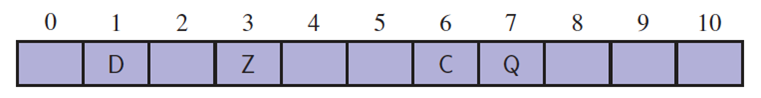
\includegraphics[width=11cm]{asp-15-pic01.png}
  \end{center}
\end{frame}

\begin{frame}[fragile]
  \frametitle{Kreiranje objekata}
  \begin{itemize}
    \item u Python programu svi objekti se čuvaju u delu memorije koji 
    se zove \myred{memory heap} ili Python heap -- ne treba mešati sa 
    strukturom podataka koja se zove heap
    \item šta se dešava kada izvršimo nešto kao:
\begin{minted}[linenos=false]{python}
w = Widget()
\end{minted}
    \item kreira se nova instanca klase i skladišti se negde na heapu
  \end{itemize}
\end{frame}

\begin{frame}[fragile]
  \frametitle{Lista slobodnih blokova}
  \begin{itemize}
    \item memorijski heap je podeljen u \myred{blokove} -- kontinualne 
    ,,parčiće`` memorije koji mogu biti fiksne ili promenljive veličine
    \item mora biti moguće brzo zauzimanje memorije za nove objekte
    \item jedno popularno rešenje -- čuvanje slobodnih ,,rupa`` u heapu
    u povezanoj listi, zvanoj \myred{lista slobodnih blokova}
    \item odlučivanje kako dodeljivati blokove iz liste slobodnih 
    prilikom zauzimanja (alokacije) memorije je deo \myred{upravljanja
    memorijom}
  \end{itemize}
\end{frame}

\begin{frame}[fragile]
  \frametitle{Upravljanje memorijom}
  \begin{itemize}
    \item postoji više načina za alokaciju memorije na heapu koji 
    minimizuju fragmentaciju
    \begin{itemize}
      \item \myred{best fit}: pronađi u celoj listi onaj blok čija 
      veličina je najbliža traženoj veličini 
      \item \myred{first fit}: kreni od početka liste i pronađi prvi
      blok koji je dovoljno velik
      \item \myred{next fit}: traži se prvi sledeći dovoljno veliki blok
      počevši od prethodne pozicije; lista je cirkularna
      \item \myred{worst fit}: pronađi najveći slobodan blok
    \end{itemize}
  \end{itemize}
\end{frame}

\begin{frame}[fragile]
  \frametitle{Sakupljanje đubreta}
  \begin{itemize}
    \item \myred{garbage collection}: proces otkrivanja ,,ustajalih`` 
    objekata, oslobađanje memorije koju ti objekti zauzimaju, i vraćanje 
    toga u listu slobodnih blokova
    \item da bi program mogao da pristupi objektu, mora imati referencu
    na njega (direktnu ili indirektnu)
    \begin{itemize}
      \item takvi objekti su \myred{živi} objekti
    \end{itemize}
    \item živi objekti koji su direktno dostupni (postoji promenljiva
    koja sadrži referencu na njih) su \myred{korenski objekti}
    \item \myred{indirektna referenca} na živi objekat je referenca koja
    se nalazi u nekom drugom živom objektu
  \end{itemize}
\end{frame}

\begin{frame}[fragile]
  \frametitle{Brojanje referenci}
  \begin{itemize}
    \item \myred{reference counting}: svaki objekat ima uz sebe i brojač
      referenci na sebe; brojač se ažurira prilikom operacija dodele
      vrednosti
    \item kada brojač padne na nulu, objekat može da se ukloni jer je
      nedostupan
    \item ali šta kada dva objekta imaju reference jedan na drugog, a
      nisu dostupni spolja (\myred{cirkularne reference})?
  \end{itemize}
\end{frame}

\begin{frame}[fragile,shrink]
  \frametitle{Python i brojanje referenci}
\begin{minted}[linenos=false]{python}
>>> import sys
>>> a = 'test'
>>> b = [a]
>>> c = {'key': a}
>>> sys.getrefcount(a)
4
>>> 
\end{minted}
\begin{itemize}
  \item referenca \texttt{a}
  \item referenca u listi \texttt{b}
  \item referenca u rečniku \texttt{c}
  \item referenca u parametru funkcije \texttt{getrefcount} prilikom poziva :)
\end{itemize}
\end{frame}

\begin{frame}[fragile]
  \frametitle{Cirkularne reference}
  \begin{itemize}
    \item šta kada dva objekta imaju reference jedan na drugog, a
      nisu dostupni spolja (\myred{cirkularne reference})?
    \item ili objekat ima referencu na samog sebe?
  \end{itemize}
\begin{minted}[linenos=false]{python}
>>> class MyClass:
...     pass
...
>>> a = MyClass()
>>> a.obj = a
>>> del a
\end{minted}
\end{frame}

\begin{frame}[fragile,shrink]
  \frametitle{Generational garbage collection}
  \begin{itemize}
    \item GC prati sve objekte u memoriji
    \item svaki novi objekat počinje život u ,,prvoj generaciji``
    \item kada se pokrene GC proces i objekat preživi, seli se u
      narednu (drugu) generaciju
    \item svaka generacija ima limit na broj objekata koji može da primi
    \item Python ima 3 generacije za GC
    \item statistika kaže: većina objekata u programu su kratkog veka
  \end{itemize}
\begin{minted}[linenos=false]{python}
>>> import gc
>>> gc.get_threshold()
(700, 10, 10)
>>> gc.get_count()
(445, 3, 3)
>>> gc.collect()
115
>>> gc.get_count()
(24, 0, 0)
\end{minted}
\end{frame}

\begin{frame}[fragile]
  \frametitle{Java: mark-and-sweep algoritam}
  \begin{itemize}
    \item svakom objektu dodeljena je oznaka (\myred{mark}) da li je
    objekat živ
    \item kada odlučimo da je potrebno skupljati đubre, \textbf{zaustavimo sve
    druge aktivnosti} i 
    \begin{itemize}
      \item ukinemo mark za sve objekte na heapu
      \item prođemo kroz sve module i sve korenske objekte označimo kao žive
      \item odredimo da li su ostali objekti dostupni preko korenskih objekata -- pretragom grafa po dubini
    \end{itemize}
  \end{itemize}
\end{frame}

\begin{frame}[fragile]
  \frametitle{Hijerarhija memorije}
  \begin{itemize}
    \item računari imaju hijerarhiju sa različitim vrstama memorije
    \item nivoi hijerarhije se razlikuju po veličini i udaljenosti od procesora
    \begin{itemize}
      \item najbliži su interni \myred{registri} procesora; pristup je vrlo brz ali ih ima vrlo malo
      \item drugi nivo: \myred{cache} memorija
      \item treći nivo: \myred{operativna} memorija (RAM)
      \item četvrti nivo: \myred{spoljašnja} memorija (diskovi)
    \end{itemize}
  \end{itemize}
  \begin{center}
    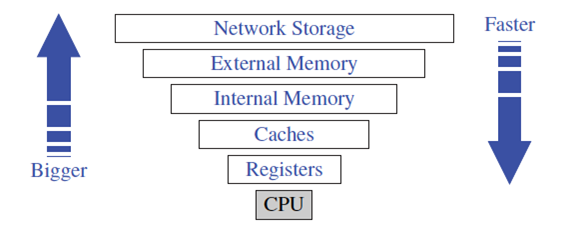
\includegraphics[width=8cm]{asp-15-pic02.png}
  \end{center}
\end{frame}

\begin{frame}[fragile]
  \frametitle{Virtuelna memorija}
  \begin{itemize}
    \item \myred{virtuelna memorija}: adresni prostor velik kao 
    kapacitet spoljne memorije
    \item stranice se premeštaju iz spoljne u operativnu memoriju kada 
    su potrebne
    \begin{itemize}
      \item virtuelna memorija ukida ograničenje veličine operativne 
      memorije
    \end{itemize}
    \item koji deo čuvati u operativnoj memoriji: \myred{caching}
    \item zahvaljujući \myred{vremenskoj lokalnosti}
    \item učitavanjem stranice u operativnu memoriju nadamo se da će ona
    biti uskoro potrebna
    \item i da ćemo moći brzo da odgovorimo na sve zahteve za tom
    stranicom u bliskoj budućnosti
  \end{itemize}
\end{frame}

\begin{frame}[fragile]
  \frametitle{Strategije zamene blokova u operativnoj memoriji}
  \begin{itemize}
    \item kada se traži nova stranica a operativna memorija je popunjena
    moramo izbaciti neku postojeću stranicu
    \item strategije za \myred{page replacement}
    \begin{itemize}
      \item LIFO
      \item FIFO
      \item random
    \end{itemize}
  \end{itemize}
\end{frame}

\begin{frame}[fragile]
  \frametitle{Random strategija}
  \begin{itemize}
    \item izaberi stranicu koju ćeš izbaciti slučajnim putem
    \begin{itemize}
      \item traje $O(1)$
      \item ali ne pokušava da iskoristi vremensku lokalnost
    \end{itemize}
  \end{itemize}
  \begin{center}
    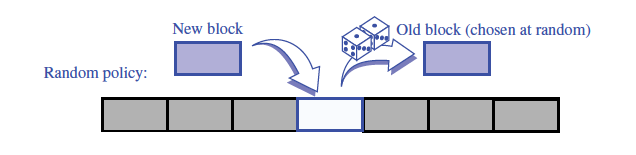
\includegraphics[width=10cm]{asp-15-pic03.png}
  \end{center}
\end{frame}

\begin{frame}[fragile]
  \frametitle{FIFO strategija}
  \begin{itemize}
    \item jednostavna za implementaciju -- potreban je red koji čuva 
    reference na stranice u kešu
    \begin{itemize}
      \item stranice se dodaju u red prilikom učitavanja
      \item kada treba izbaciti stranicu, uklanja se prva stranica iz 
      reda -- $O(1)$
      \item pokušava da iskoristi vremensku lokalnost
    \end{itemize}
  \end{itemize}
  \begin{center}
    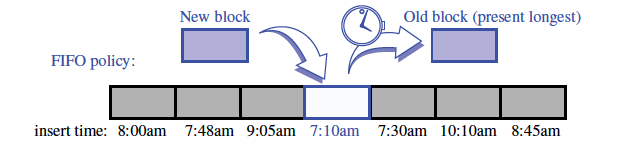
\includegraphics[width=10cm]{asp-15-pic04.png}
  \end{center}
\end{frame}

\begin{frame}[fragile]
  \frametitle{LRU strategija}
  \begin{itemize}
    \item \myred{least recently used} -- najdavnije korišćena stranica
    \begin{itemize}
      \item odlična politika ali implementacija može biti komplikovana
      \item potreban je adaptivni red sa prioritetom
      \item ako se implementira kao sortirana sekvenca pomoću povezane
      liste, uklanjanje je $O(1)$
    \end{itemize}
  \end{itemize}
  \begin{center}
    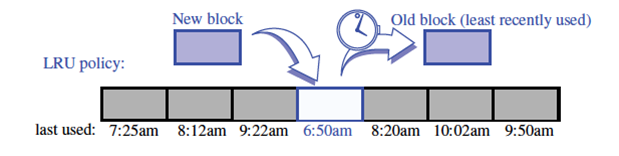
\includegraphics[width=10cm]{asp-15-pic05.png}
  \end{center}
\end{frame}

\section[B-stabla]{B-stabla}

\begin{frame}[fragile]
  \frametitle{Blokovi na disku}
  \begin{itemize}
    \item čuvamo veliku kolekciju elemenata koja ne može stati u 
    operativnu memoriju
    \item spoljnu memoriju smo podelili na \myred{disk blokove} -- red 
      veličine 8KB
    \item prenos bloka između spoljne i operativne memorije je 
    \myred{disk transfer} ili \myred{I/O}
    \item velika razlika između vremena pristupa operativnoj i spoljnoj 
    memoriji
    \item $\Rightarrow$ želimo da minimizujemo broj disk transfera da
    bismo izvršili pretragu ili ažuriranje
    \item ovaj broj zovemo \myred{I/O kompleksnost} algoritma
  \end{itemize}
\end{frame}

\begin{frame}[fragile]
  \frametitle{(a,b) stablo}
  \begin{itemize}
    \item možemo predstaviti mapu za pretragu pomoću n-arnog stabla
    \item \myred{(a,b) stablo} predstavlja uopštenje (2,4) stabla
    \begin{itemize}
      \item (a,b) stablo je n-arno stablo u kome svaki čvor ima između
      $a-1$ i $b-1$ dece
    \end{itemize}
    \item podešavanjem parametara $a$ i $b$ u odnosu na veličinu disk 
    bloka možemo postići dobre I/O performanse
  \end{itemize}
\end{frame}

\begin{frame}[fragile]
  \frametitle{(a,b) stablo}
  \begin{itemize}
    \item \myred{(a,b) stablo} gde su $a$ i $b$ celobrojni parametri 
    takvi da je $2\leq a\leq (b+1)/2$ je n-arno stablo pretrage sa
    sledećim osobinama
    \begin{itemize}
      \item \myred{veličina}: svaki interni čvor osim korena ima 
      najmanje $a$ dece; koren ima najviše $b$ dece
      \item \myred{dubina}: svi listovi imaju istu dubinu
    \end{itemize}
  \end{itemize}
\end{frame}

\begin{frame}[fragile]
  \frametitle{Visina (a,b) stabla}
  \begin{itemize}
    \item visina (a,b) stabla sa $n$ elemenata je
    \begin{itemize}
      \item $\Omega(\log n/\log b)$
      \item $O(\log n/\log a)$
    \end{itemize}
  \end{itemize}
\end{frame}

\begin{frame}[fragile]
  \frametitle{Pretraga i ažuriranje u (a,b) stablu}
  \begin{itemize}
    \item pretraga se odvija kao u n-arnom stablu
    \item dodavanje slično (2,4) stablu
    \begin{itemize}
      \item overflow nastupa kada se dodaje element u $b$-čvor
      \item čvor se deli pomeranjem median vrednosti u roditelja i zamenom čvora sa
      dva nova $(b+1)/2$-čvora
    \end{itemize}
    \item uklanjanje slično (2,4) stablu
    \begin{itemize}
      \item underflow nastupa kada se ukloni element iz $a$-čvora
      \item ako je brat $a$-čvor radi se fuzija
      \item ako brat nije $a$-čvor radi se transfer
    \end{itemize}
  \end{itemize}
\end{frame}

\begin{frame}[fragile]
  \frametitle{B-stablo}
  \begin{itemize}
    \item najpoznatija struktura za čuvanje mape u spoljnoj memoriji
    \item \myred{B-stablo} reda $d$ je (a,b) stablo za $a=d/2$ i $b=d$
  \end{itemize}
  \begin{center}
    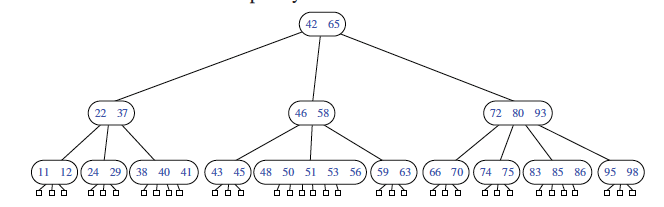
\includegraphics[width=11cm]{asp-15-pic07.png}
  \end{center}
\end{frame}

\begin{frame}[fragile]
  \frametitle{I/O složenost B-stabla}
  \begin{itemize}
    \item B-stablo sa $n$ čvorova ima I/O složenost $O(\log_{B}n)$ za pretragu
    i ažuriranje, i troši $O(n/B)$ blokova, gde je $B$ veličina bloka
  \end{itemize}
\end{frame}

\end{document}
